\section{Architekturstile}
\label{sec:architekturstile}
    \subsection{Monolith}
    \label{subsec:monolith}

    % Einleitung zu Monolithen
    Unter den Softwarearchitekturen ist der Monolith ein weit verbreiteter und genutzter Architekturstil. Der Monolith mit seiner Analogie zu einem einheitlichen, massiven Stein, birgt gewisse Vor- und Nachteile gegenüber anderen Architekturen. Diese, als auch der grundlegende Aufbau einer solchen Architektur, werden im Folgenden erläutert.

    % Aufbau eines Monolithischen Systems
    Ein monolithisches System vereint jegliche verwendete Technologien in einem einzigen Prozess \parencites{newman2019monolith}[S. 21]{gallipeau2018microservices}. Laut Takai entsteht dadurch \glqq [...] ein einschichtiges, untrennbares und technologisch homogenes System, das verschiedene Services in sich vereint\grqq{} \parencite[S. 17]{takai2017architektur}. Newman unterscheidet zwischen vier verschiedenen Arten des Monolithen:%

    \begin{itemize}
        \item Einzelprozess-Monolith
        \item Modularer Monolith
        \item Verteilter Monolith
        \item Drittanbieter-Black-Box-Systeme
    \end{itemize}
    
    \subsubsection{Einzelprozess-Monolith}
    % Einzelprozess-Monolith - Erläuterung
    Der \emph{Einzelprozess-Monolith} ist die am häufigsten auftretende Form der monolithischen Softwarearchitektur. Wie vorher schon durch Takai beschrieben, besitzt dieser die Eigenschaft verschiedene Technologien in sich und unter einem Prozess zu vereinen. Somit bietet der Einzelprozess-Monolith den Ursprung des monolithischen Architekturstils. Wie weiter oben aufgelistet, entwickeln sich aus diesem weitere Varianten, die für die Entwicklung eines Softwareproduktes genutzt werden können.
    
    Wenn zukünftig in dieser Arbeit der Monolith benannt wird, so ist damit der Einzelprozess-Monolith gemeint, da dieser zu der bekanntesten Art der monolithischen Softwarearchitektur gehört. Eine derartige Architektur wird in \autoref{fig:monolith_scribble} skizziert.
    
    \begin{figure}[!t]
        \vspace{.02\textheight}
        \centering
        \tikzset{
            ent/.style={
                rectangle,
                fill=red!20,
                draw=red,
                semithick
            },
            db/.style={
                cylinder,
                fill=orange!10,
                draw=orange,
                semithick,
                inner sep=3mm,
                shape border rotate=90,
                aspect=0.25
                },
            typetag/.style={
                rectangle,
                draw=black!50,
                anchor=west
            }
        }
        \begin{tikzpicture}[node distance=2cm]
            \path
                node (gui) at (5,10) {GUI}
                node[below=2mm of gui] (bus)  {Geschäftslogik}
                node[below=2mm of bus] (dba) {Persistenz}
                node[below=2mm of dba] (etc) {etc...}
                node[minimum width=.4\textwidth, minimum height=4cm,ent, behind path,fit={(gui) (bus) (dba) (etc)},inner sep=10pt](mon) {};

            \node[db,right=of mon] (db) {Datenbank};
            \draw[->, very thick] (mon) edge node[above]{Zugriff auf} (db);

            \draw[line width=1pt,black,decorate,decoration={amplitude=7pt,brace,mirror}] ([yshift=1.2mm,xshift=2mm]mon.north east) -- ([yshift=1.2mm,xshift=-2mm]mon.north west);
            \node[above=7mm of mon,anchor=center]{Monolith};
        \end{tikzpicture}
        \caption{Skizze eines Einzelprozess-Monolithen \parencite{newman2019monolith}}
        \label{fig:monolith_scribble}
    \end{figure}

    \subsubsection{Modularer Monolith}
    Eine Variation des Einzelprozess-Monolithen ist ein \emph{modularer Monolith}. Anders als bei einem gewöhnlichen Monolithen, wird dieser zur Entwicklungszeit in Module untergliedert, welche unabhängig voneinander weiterentwickelt werden können. Zum Distributieren der entstehenden Software müssen diese Module jedoch wieder in einen einzigen Prozess zusammengefügt werden. Solange ein modularer Monolith klar getrennte Module aufweist, kann dies für ein Unternehmen gut funktionieren. Es ist hierbei zu beachten, dass die Datenbank, genau wie der modulare Monolith selbst, in dessen Module dekomponiert werden soll. Laut Newman wird dies allerdings nur selten realisiert. \autoref{fig:modularer_monolith} skizziert den grundlegenden Aufbau eines modularen Monolithen \parencite{newman2019monolith}.
    
    Als Beispiel fungiert hierfür das Unternehmen \emph{Shopify}, welches einen gewöhnlichen Monolithen in einen modularen Monolithen umstrukturieren konnte. Ersteres führte nach Wachstum von Software und Unternehmen zu Problemen in den Bereichen Wartbarkeit, Testbarkeit und Erweiterbarkeit. Der Übergang von einem Monolithen zu einer Microservice-Architektur wäre für Shopify zu aufwändig gewesen, da dies eine Neuentwicklung des Produktes erfordert hätte \parencite{westeinde2019deconstructmonolith}.

    \begin{figure}[ht]
        \vspace{.02\textheight}
        \centering
        \begin{tikzpicture}[node distance=0cm]
            \tikzset{
            ent/.style={
                rectangle,
                fill=red!20,
                draw=red,
                semithick
            },
            db/.style={
                cylinder,
                fill=orange!10,
                draw=orange,
                semithick,
                inner sep=3mm,
                shape border rotate=90,
                aspect=0.25
                },
            typetag/.style={
                rectangle,
                draw=black!50,
                anchor=west
            }
        }
        \node[ent, minimum height=2cm, minimum width=.3\textwidth] (modmonA) {Modul A};    
        \node[ent, minimum height=2cm, minimum width=.3\textwidth, below=of modmonA] (modmonB) {Modul B};
        \node[ent, minimum height=2cm, minimum width=1.78cm, right=of modmonA] (modmonC) {Modul C};
        \node[ent, minimum height=1cm, minimum width=1.78cm, below=of modmonC] (modmonD) {Modul D};
        \node[ent, minimum height=1cm, minimum width=1.78cm, below=-0.5pt of modmonD] (modmonE) {Modul E};
        
        \node[db,right=2cm of modmonC, align=center] (dbC) {Datenbank\\Modul C};
        \draw[->, very thick] (modmonC) edge node[above]{Zugriff auf} (dbC);
        \node[db,right=4cm of modmonD, align=center] (dbD) {Datenbank\\Modul D};
        \draw[->, very thick] (modmonD) edge node[above]{Zugriff auf} (dbD);
        \node[db,right=6.2cm of modmonE, align=center] (dbE) {Datenbank\\Modul E};
        \draw[->, very thick] (modmonE) edge node[above]{Zugriff auf} (dbE);

        \node[fit= (modmonA) (modmonB) (modmonC) (modmonD) (modmonE)](group){};
        \draw[line width=1pt,black,decorate,decoration={amplitude=7pt,brace,mirror}] (group.north east) -- (group.north west);
        \node[above=6mm of group,anchor=center]{Modularer Monolith};
        
        \end{tikzpicture}
        \caption{Skizze eines modularen Monolithen \parencite{newman2019monolith}}
        \label{fig:modularer_monolith}
    \end{figure}

    \subsubsection{Verteilter Monolith}
    \label{subsubsec:distributedmonolith}
    Der verteilte Monolith ist weniger ein Architekturstil, als vielmehr ein unerwünschtes Artefakt, welches aus nicht eingehaltenen, spezifischen Entwurfsprinzipien der \gls{ac-soa} entsteht. Die Kernessenz von SOA besteht darin verschiedene Services zu gestalten, welche jeweils als eigene Prozesse unabhängig voneinander existieren und agieren können. SOA wird in \autoref{subsec:soa} weiter erläutert \parencites{newman2019monolith}{erl2005soa}.
    
    Verteilte Monolithen entstehen oftmals in Umgebungen, in welchen zu wenig Zeit und Fokus in die Abstraktion von \emph{Services} als auch deren Kohäsion von Geschäftslogik investiert wurde. Dadurch entstehen mehrere Services mit verwischten \emph{Servicegrenzen}, wodurch eine stark gekoppelte Architektur entsteht, in welcher eine Veränderung in einem Service das ganze System beeinflussen kann. Im Idealfall sollte nur der veränderte Service von dessen Modifizierung beeinflusst werden. Beispielsweise sollte ein \gls{ac-soa} System, bestehend aus einem \emph{User-Service}, \emph{Renderjob-Service} und \emph{Download-Service}, nicht zusammenbrechen sobald der User-Service modifiziert wurde. Der modifizierte Service selbst kann abstürzen, jedoch sollte in einem solchen Fall der Rest des Systems, bestehend aus dem Renderjob-Service und dem Download-Service, fortbestehen können. Da ein Entwurfsprinzip von SOA die Partitionierung von Ressourcen und somit die lose Kopplung von Komponenten eines Systems ist, kann ein verteilter Monolith daher nicht die Versprechen von SOA einhalten \parencites{newman2019monolith}{richardson2018mspatterns}.
    \clearpage

    \subsubsection{Drittanbieter-Black-Box-Systeme}
    Als letzte Art des Monolithen gelten laut Newman Drittanbieter-Black-Box-Systeme. Diese sind extern entwickelte Services. Solche können sowohl als Open Source Systeme in der eigenen Infrastruktur, als auch als \gls{ac-saas} Produkte über eine \emph{API} oder ein \emph{SDK} eingesetzt werden. Beispiele für solche Systeme wären der Objektspeicher \emph{MinIO} und Google's \gls{ac-baas}, \emph{Firebase}. MinIO gewährt dabei als Open Source Produkt Einblick in dessen Quellcode welchen man modifizieren kann, auch wenn dies mit einem gewissen Aufwand verbunden ist. Somit läuft man gerade bei Google's Firebase Gefahr, dass dieses BaaS Produkt ein Monolith ist, der eine typische Black-Box darstellt. Dort wird über eine API verdeutlicht, welche Funktionalität die Black-Box bereitstellt, jedoch nicht deren Art und Weise um die Funktionalität zu erfüllen. Dies ist besonders dann ein Problem, wenn für die entwickelte Software bestimmte Konditionen herrschen. Ein Beispiel dafür wäre ein Wert, der in einem bestimmten Typ zurückgegeben werden muss. Die externen Services MinIO und Firebase werden für diese Arbeit genutzt und dementsprechend in dem \autoref{sec:verwendete_technologien} weiter erläutert \parencite{newman2019monolith}.

    \subsubsection{Vor- und Nachteile von Monolithen}
    Monolithen werden oftmals als problematisch eingestuft, obwohl diese Art der Softwarearchitektur ein valider Stil zum Entwickeln von Software ist. Vorteile von Monolithen finden sich durch die zentralisierte Codebasis in der Reduzierung der Komplexität des \gls{gl-devops}-Bereichs wieder.
    
    Eine monolithische Java Webapplikation kann zum Beispiel mithilfe einer einzelnen \gls{ac-war} Datei auf einem Server installiert werden. Die Applikation benötigt also nur einen Kompilierungs- und Installationsprozess. Im Falle eines verteilten Systems müssen allerdings, wie in \autoref{subsec:soa} und \autoref{subsec:microservices} beschrieben, mehrere solcher Kompilierungen und Installationen durchgeführt werden, da jeder Service als eigenständiges System zu betrachten ist. Ein Monolith kann auch zu simpleren Workflows für Entwickler führen. Da der ganze Code für einen Monolithen in einem Prozess zu finden ist, können auftretende Fehler in verschiedenen Teilbereichen der Software in der selben Codebasis behoben werden, während sich der Kompiliervorgang deswegen nicht ändern muss. So lassen sich signifikante Änderungen an einer monolithischen Software effizient vornehmen. Verteilte Systeme hingegen benötigen für jeden Service einen individuell angepassten Kompiliervorgang, da diese einen eigenen Technologie-Stack besitzen können. Der Monolith beschreibt ebenfalls einen klaren Weg zum Testen von Software. So kann eine Monolithische Software mithilfe des \gls{ac-e2e} Verfahrens in jedem ihrer Teilbereiche getestet werden. Da sich diverse Teile der Software hier in einem Prozess wiederfinden, kann zum E2E Testen immer sofort die komplette Software getestet werden. Ein weiterer Vorteil liegt bei der Simplizität der Skalierung eines Monolithen vor. Da ein Monolith nur aus einem Prozess besteht, kann auch nur dieser als ein solcher skaliert werden. Deshalb können bei monolithischen Webapplikationen mit Problemen bei der Performance mehrere Instanzen dieser installiert werden. Ein \gls{gl-loadbalancer} könnte zwischen diesen dann einkommende \gls{ac-http}-Anfragen verteilen. Diese Vorteile sind besonders für kleinere Softwareprojekte gegeben \parencites{newman2019monolith}{richardson2018mspatterns}[S. 24]{namiot2014micro}.

    Auch wenn kleinere Monolithen eine geringe Komplexität für einzelne Entwickler oder kleinere Entwicklerteams bergen, so kann diese proportional zur Größe des Monolithen wachsen. Somit besitzen größere Monolithen wiederum einige Nachteile, welche im nächsten Abschnitt aufgezählt werden.

    \begin{figure}[ht]
        \vspace{.02\textheight}
        \centering
        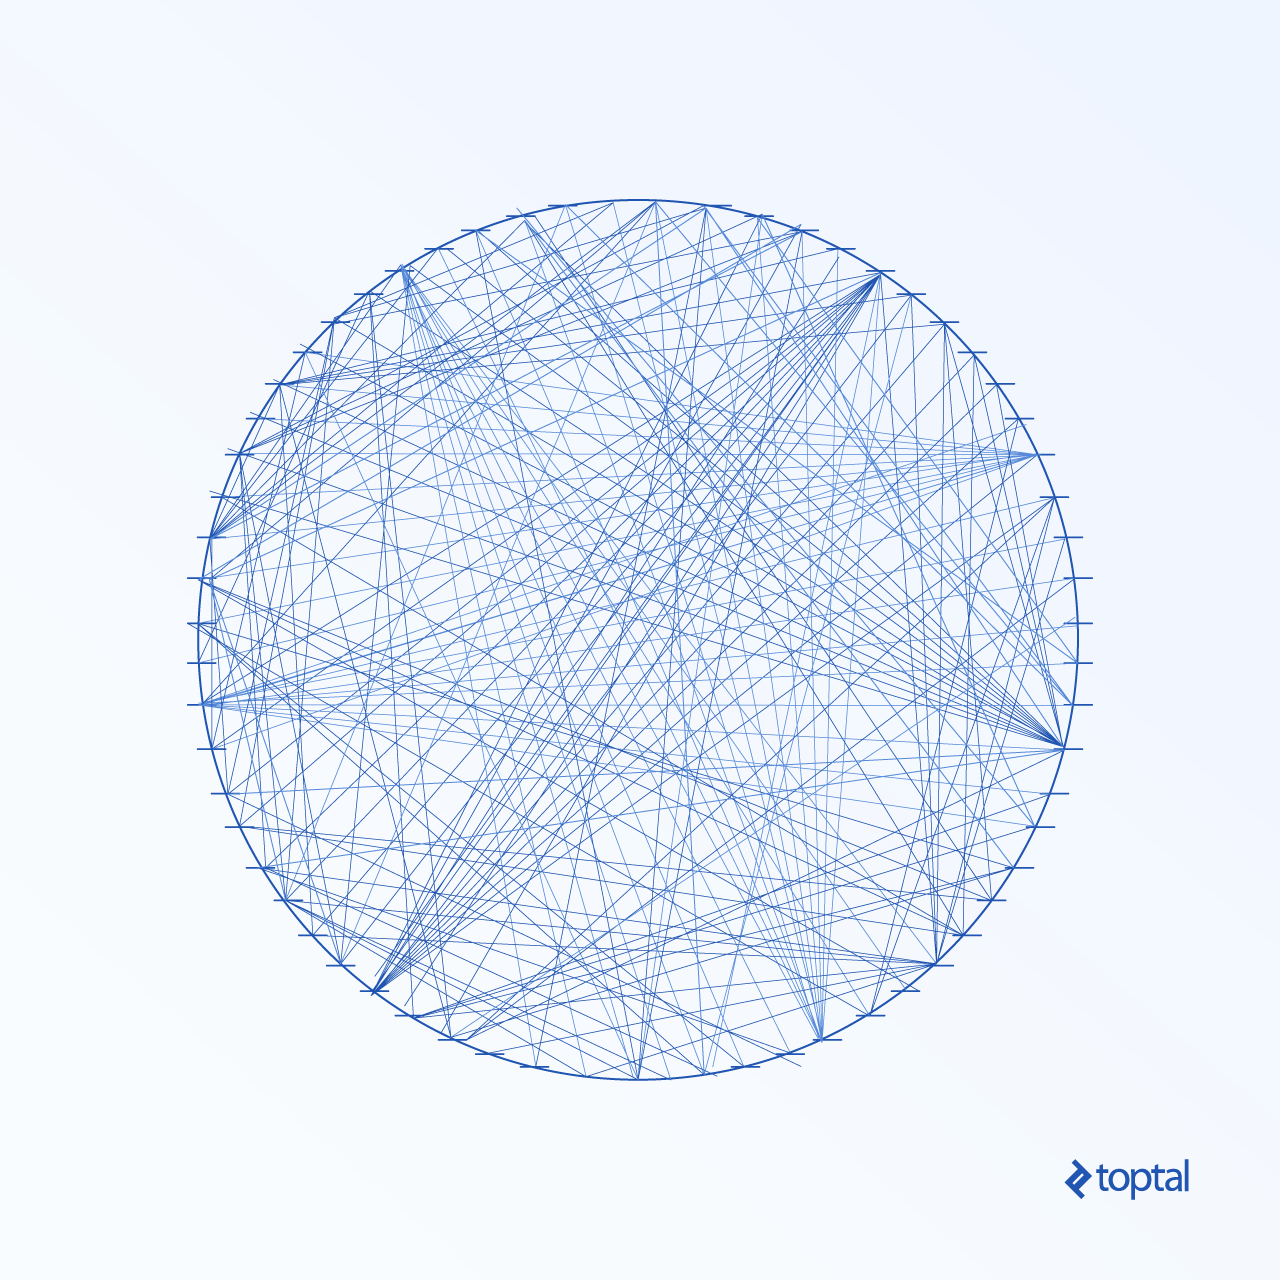
\includegraphics[width=.5\textwidth]{res/img/bigballofmud.png}
        \caption{Darstellung der grenzenlosen Kommunikation der Komponenten eines \emph{Big Ball of Mud} \parencite{Gadzinowski2017bigballofmud}}
        \label{fig:bigballofmud}
    \end{figure}

    Bei größeren Monolithen spricht man umgangssprachlich von einem \emph{Big Ball of Mud} \parencite[S. 17]{takai2017architektur}. Ein solches System besitzt keine inneren Grenzen, sodass weit entfernte Komponenten des Systems auf direktem Weg Informationen teilen. Eine solche Kommunikation ist in \autoref{fig:bigballofmud} dargestellt. Dies geht laut Foote und Yoder so weit, dass später wichtige Informationen im globalen Umfang oder sogar dupliziert im Code vorhanden sind \parencite{footeyoder1997bigballofmud}. Jene Entwickler eines Monolithen müssen einen Großteil der Codebasis verstehen, damit an dieser Änderungen vorgenommen werden können. Die grenzenlose Kommunikation der Systemkomponenten bei einem großen Monolithen jedoch erschwert ein solches Vorhaben. Für neue Entwickler wird es zunehmend schwieriger sich in das System einzuarbeiten, was ein immer weniger produktives Unternehmen zur Folge hat. Das Verwischen dieser Systemgrenzen führt ebenfalls dazu, dass Entwickler in verschiedenen Teilbereichen der Software arbeiten müssen. Dies führt oft zu Unklarheiten bei den Entwicklern bezüglich der Zugehörigkeit und Zuständigkeit des geschriebenen Codes. Auch wenn ein modularer Monolith seine Systembereiche voneinander abtrennt, kann keiner dieser Bereiche unabhängig voneinander skaliert werden. Nimmt man sich wieder das Beispiel des verteilten Monolithen mit den Komponenten \emph{User-Service}, \emph{Renderjob-Service} und \emph{Download-Service}, so könnte man hier jenen Service, der droht überstrapaziert zu werden, mit einer weiteren Instanz ausstatten. Im Falle des Monolithen ist man allerdings durch die starke Kopplung der Komponenten gezwungen eine weitere Instanz der kompletten Software zu starten. \autoref{fig:monservscaling} stellt die Art der Skalierung für beide Architekturstile dar. Dabei ist zu beachten, dass der User-Service, Renderjob-Service und Download-Service ein verteiltes System komponieren, während der Monolith diese Services stark gekoppelt in sich vereint und deshalb nicht in seinen Komponenten dargestellt wird. Die starke Kopplung eines Monolithen wird diesem im Falle eines Updates zum Verhängnis, denn für jedes Update muss die komplette Applikation neu veröffentlicht werden. Mit einem wachsenden Monolithen wird es schwieriger für das Entwicklerteam die Entwicklungsframeworks zu ändern, weshalb ein monolithisches Projekt zunehmend unflexibel wird \parencites{richardson2018mspatterns}[S. 24]{namiot2014micro}[S. 21--22]{gallipeau2018microservices}.

    \begin{figure}[!ht]
        \vspace{.02\textheight}
        \centering
        %\resizebox{.67\textwidth}{!}{
            \begin{tikzpicture}
                \tikzset{
                    mon/.style={
                    rectangle,
                    fill=red!20,
                    draw=red,
                    semithick
                    },
                ser/.style={
                    rectangle,
                    fill=blue!20,
                    draw=blue,
                    semithick
                },
                db/.style={
                    cylinder,
                    fill=orange!10,
                    draw=orange,
                    semithick,
                    inner sep=3mm,
                    shape border rotate=90,
                    aspect=0.25
                    },
                typetag/.style={
                    rectangle,
                    draw=black!50,
                    anchor=west
                },
                client/.style={
                    diamond,
                    semithick,
                    draw=yellow!70!black,
                    fill=yellow!30
                }
            }
            %% Client
            \node[client] (client) at (0,0) {Client};

            %% Services
            \node[ser, right=5cm of client, minimum width=3.3cm, minimum height=1.5cm] (ser1) {};
            \node[ser, right=5cm of client, minimum width=3.3cm, minimum height=1.5cm, xshift=2mm, yshift=-2mm] (ser12) {};
            \node[ser, right=5cm of client, minimum width=3.3cm, minimum height=1.5cm, xshift=4mm, yshift=-4mm] (ser13) {Renderjob-Service};
            
            % Renderjob-Services Group
            \node[fit=(ser1)(ser12)(ser13)](sergroup){};
            \draw[line width=1pt,black,decorate,decoration={amplitude=7pt,brace}]
            (sergroup.north east) -- (sergroup.south east);
            \node[right=of sergroup,anchor=center,rotate=90, align=left]{Einzelner Service\\muss skaliert werden};

            % Renderjob-Services Group Comment
            \node[ser, above=2mm of ser1, minimum width=3.3cm, minimum height=1.5cm] (ser2) {User-Service};
            \node[ser, below=6mm of ser1, minimum width=3.3cm, minimum height=1.5cm] (ser3) {Download-Service};

            %% Monoliths
            \node[mon, above=of ser2, minimum width=1.8cm, minimum height=1.8cm] (mon1) {};
            \node[mon, above=of ser2, minimum width=1.8cm, minimum height=1.8cm, xshift=2mm, yshift=-2mm] (mon2) {};
            \node[mon, above=of ser2, minimum width=1.8cm, minimum height=1.8cm, xshift=4mm, yshift=-4mm] (mon3) {Monolith};

            % Monoliths Group Comment
            \node[fit=(mon1)(mon2)(mon3)](mongroup){};
            \draw[line width=1pt,black,decorate,decoration={amplitude=7pt,brace}]
    (mongroup.north east) -- (mongroup.south east);
            \node[right=of mongroup,anchor=center,rotate=90, align=left]{Ganze Applikation\\muss skaliert werden};

            % client -> Monolith
            \draw[->, very thick] (client) -- ++(0,1) node[above, yshift=1.5cm, rotate=90]{HTTP Anfragen} |- node[above, xshift=5.7cm]{viel Last} (mon1);
            % client -> Renderjob-Service
            \draw[->, very thick] (client) -- node[above, xshift=1.2cm, yshift=0.7mm]{viel Last} (ser1);
            % client -> User-Service 
            \draw[->, very thick] (client) -- ++(3.8,0) node[above, xshift=-1.5cm]{HTTP Anfragen} |- node[above, xshift=1cm]{wenig Last} (ser2); 
            % client -> Download-Service
            \draw[->, very thick] (client) -- ++(3.8,0) |- node[above, xshift=1cm]{wenig Last} (ser3); 
            \end{tikzpicture}
            %} %resizebox end
            \caption{Gegenüberstellung der Skalierungsform eines Monolithen und eines verteilten Systems}
            \label{fig:monservscaling}
        \end{figure}

    %Nachdem nun der monolithische Architekturstil erläutert und dessen Vor- und Nachteile herausgestellt wurden, widmet sich der nächste Unterabschnitt der \acrfull{ac-soa}.

    \subsection{SOA}
    \label{subsec:soa}
    Im Jahr 2000 kam der Architekturstil der \acrlong{ac-soa} auf und bietet eine Alternative zur monolithischen Architektur. Dieser Stil \glqq [...] wurde durch das Platzen der Dotcom-Blase in 2001 beflügelt, als man feststellte, dass die Serviceorientierung Marktvorteile bietet [...]\grqq{} \parencite[S. 12]{takai2017architektur}. SOA gilt als ein Vorreiter von Microservices, weshalb sich zwischen diesen beiden Stilen auch einige Ähnlichkeiten feststellen lassen.
    
    Im Gegensatz zum Monolithen achtet man bei diesem Stil darauf mehrere Systeme zu entwickeln, welche isoliert voneinander existieren und miteinander kommunizieren können. Dabei stellt ein Service die primäre Quelle der Geschäftslogik dar. Die Kommunikation der Services findet nach Regeln eines Vertrages statt, wobei es keine Rolle spielt, welche Technologie die kommunizierenden Services benutzen, um ihre Anwendungsbereiche zu erfüllen \parencites[S. 12]{takai2017architektur}{erl2005soa}{newman2019monolith}[S. 22]{gallipeau2018microservices}.
    %\clearpage
    
    Laut Takai erwuchs \gls{ac-soa} aus zwei Strömungen:
    \begin{itemize}
        \item Objektorientierte Analyse und Design
        \item Webservices
    \end{itemize}

    Ersteres schulte Softwarearchitekten ihre Systeme so zu entwerfen, damit diese erweiterbar, wiederverwendbar, flexibel und robust sind, um ihre Geschäftsziele genau abzudecken. Letzteres leitete die Funktionalität ein, dass Services mithilfe von genormten Kommunikationsprotokollen wie \gls{ac-http} miteinander kommunizieren können \parencite[S. 12]{takai2017architektur}.
    %\clearpage

    Laut Erl gelten für eine \gls{ac-soa} acht Entwurfsprinzipien:
    \begin{itemize}
        \item \textbf{Servicewiederverwendbarkeit}: Ein Service sollte eine potenzielle Wiederverwendbarkeit mit sich führen. Ziel ist es hierbei einen Servicekatalog zu entwickeln, in welchem Services vorhanden sind, die von verschiedenen Akteuren genutzt werden können.
        \clearpage
        
        \item \textbf{Servicevertrag}: Mithilfe eines Vertrages kann ein Service darstellen, welche Methoden seine API zur Verfügung stellt und spezifizieren, welche Art von Eingabe- und Ausgabematerial unterstützt wird. So können auch Regeln und Charakteristika des Services selbst und dessen Operationen erläutert werden. So weiß ein anfragender Service, was er von einem angefragten Service mit welcher Eingabe erhält.
        
        \item \textbf{Lose Kopplung}: Ein Service sollte beim Anfragen eines anderen Services von diesem entkoppelt bleiben. Dies wird durch Serviceverträge erreicht, da damit der anfragende Service nur mit stark eingeschränkten Parametern mit dem angefragten Service kommunizieren kann. Eine Kopplung der Services ist hierbei allerdings nicht komplett zu vermeiden.
        
        \item \textbf{Serviceabstraktion}: Services werden bei der \gls{ac-soa} als Black-Box-Services entwickelt, welche mithilfe des Servicevertrages nur ihre nötigsten Informationen veröffentlichen. Dabei spielt die Größe der darunterliegenden Infrastruktur keine Rolle.
        
        \item \textbf{Service Composability}: Services sollten so gestaltet werden, dass sie effektiv von anderen Services konsumiert werden können. Eine Komposition aus verschiedenen Services kann wiederum eine komplexe Geschäftsanwendung widerspiegeln.
        
        \item \textbf{Serviceautonomie}: In der Servicegrenze sollte jeder Service seine Operationen handlungsfrei ausüben können.
        
        \item \textbf{Servicezustandslosigkeit}: Bei einem zustandslosen Service \glqq muss ein Akteur nichts über seine Historie wissen, um eine Anfrage platzieren zu können\grqq{} \parencite[S. 13]{takai2017architektur}. Bleibt ein Service so schnell und lange wie möglich zustandslos, kann dieser die Anfragen weiterer Akteure schneller behandeln.
        
        \item \textbf{Service Discoverability}: Mithilfe einer \emph{Service-Discovery} können Services dynamisch und automatisch von anderen Services gefunden werden. Mit einem solchen Prinzip lassen sich Services besser skalieren. Service-Discovery wird in \autoref{subsec:discoverability_pattern} weiter beschrieben.
    \end{itemize}
    \parencites[S. 13--14]{takai2017architektur}{erl2005soa}
    %\clearpage

    Diese Entwurfsprinzipien nach Erl sorgen für ein System in welchem die Komponenten unabhängig voneinander agieren können. Ebenfalls werden Services wiederverwendbar und lassen sich in verschiedenen Geschäftsanwendungen nutzen. Dabei können diese über festgelegte Kommunikationsprotokolle miteinander kommunizieren und Daten versenden,\clearpage welche dann von weiteren Services konsumiert werden können. Viele dieser Entwurfsprinzipien treffen auch auf Microservices zu. Allerdings konnte \gls{ac-soa} nicht von Beginn an in der IT-Branche florieren \parencites[S. 14--15]{takai2017architektur}{erl2005soa}[S. 22]{gallipeau2018microservices}.

    Laut Takai machte \gls{ac-soa} viele Versprechen, die zu jener Zeit nicht eingehalten werden konnten. Unter anderem fehlte die Technologie, um eine solche Architektur nachvollziehbar umsetzen zu können. Jeder Service braucht seine eigene Laufzeitumgebung, was in der Zeit ohne Virtualisierung impliziert, dass für jeden Service ein Server eingekauft werden musste. Ebenfalls gab es nun Services, die von allen konsumiert wurden statt von nur einer Abteilung. Darunter litten die Performance und die Skalierbarkeit der Services, was zu einer Verlangsamung dieser führte. Takai stellt allerdings besonders heraus, dass der Fokus der Unternehmen darauf saß, schwergewichtige Standards wie das \gls{ac-soap} zu etablieren, wobei der geschäftliche Nutzen von SOA unerforscht blieb. Diese Lücke zwischen IT und Geschäft lässt sich allerdings durch \gls{ac-ddd} bei dem Entwurf eines verteilten Systems schließen \parencite[S. 16]{takai2017architektur}.

    \subsection{Microservices}
    \label{subsec:microservices}

    %% EINLEITUNG
    % Historische Einleitung zu Microservices
    Nach dem Aufstieg und Verfall von \gls{ac-soa} fiel bei einem Workshop von Softwarearchitekten in der Nähe von Wien im Jahr 2011 das erste Mal der Begriff des \emph{Microservice}. Im Mai 2012 entschied dieselbe Gruppe von Softwarearchitekten, dass der Terminus des Microservice der passendste Ausdruck für die in diesem Unterabschnitt erklärte Softwarearchitektur sei. Microservices ist zum Zeitpunkt dieser Arbeit ein noch junges Themengebiet, welches allerdings in kurzer Zeit viel Aufmerksamkeit bekommen hat \parencite{fowlerlewis2014microservices}.

    \begin{figure}[h!]
      \vspace{.01\textheight}
      \centering
      \begin{tikzpicture}
        \begin{axis}[
          scale only axis,
          height=4cm,
          width=\textwidth-1.25cm,
          date coordinates in=x,
          date ZERO=2004-05-01,
          max space between ticks=80,
          xticklabel=\year,
          ylabel = Suchinteresse,
          grid=both,
          y label style={at={(axis description cs:0,.5)},anchor=north},
          legend style={at={(0.5,-0.15)},anchor=north,legend columns=-1},
          ymin=0,
          ymax=100,
          xmin=2004-01-01,
          xmax=2020-01-01]
          \addplot [color=red, mark=none, very thick, smooth] table [x=wk, y=soa, col sep=comma] {res/data/trends/google-trends-ms-vs-soa-world.csv};
          \addplot [color=blue, mark=none, very thick, smooth] table [x=wk, y=ms, col sep=comma] {res/data/trends/google-trends-ms-vs-soa-world.csv};
          \legend{Serviceorientierte Architektur, Microservices}
        \end{axis}
      \end{tikzpicture}
      \caption{Suchinteresse an den Architekturstilen Microservices und Serviceorientierte Architektur ab 2004 im weltweiten Vergleich \parencite{googletrends2020msvssoa}}
      \label{fig:google-trends-ms-vs-soa-world}
    \end{figure}
    
    Wie \autoref{fig:google-trends-ms-vs-soa-world} zeigt, erhöhte sich die Suchanfrage in Google nach SOA stetig bis zu einem Hochpunkt im Jahr 2007. Wie in \autoref{subsec:soa} bereits vermerkt, lässt sich vermuten, dass das Platzen der Dotcom-Blase das Interesse an SOA positiv beeinflusste. Ab diesem Zeitpunkt verlor SOA kontinuierlich an Aufmerksamkeit, mit Ausnahme von vier lokalen Hochpunkten jeweils im September der Jahre 2011 bis 2014. Obwohl Microservices bis 2014 kaum Aufmerksamkeit bekamen, überholte letztenendes die Suchanfrage nach Microservices die von SOA im Jahr 2019 und macht somit diese zu einem aktuellen Diskussionsthema.
    %\clearpage

    %% HAUPTTEIL
    % Architektonische Eigenheiten verglichen mit SOA

    Oftmals werden Microservices als feinkörniges \gls{ac-soa} beschrieben, da diese sich in ihrer Grundstruktur von SOA nur geringfügig unterscheiden. Aus diesem Grund wird eine Microservice-Architektur als eine leichtgewichtige Untermenge des SOA Architekturstils angesehen. Auch wenn SOA und Microservices viele Gemeinsamkeiten aufweisen, unterscheiden sich diese doch in einigen wenigen jedoch bedeutsamen Punkten \parencites[S. 20]{takai2017architektur}[S. 584]{villamizar2015evaluating}.
    %\clearpage

    \begin{figure}[h]
      \vspace{.02\textheight}
      \centering
      \begin{tikzpicture}
        \tikzset{
        app/.style={
            rectangle,
            fill=red!20,
            draw=red,
            semithick
            },
        ser/.style={
            rectangle,
            fill=blue!20,
            draw=blue,
            semithick
            },
        db/.style={
            cylinder,
            fill=orange!10,
            draw=orange,
            semithick,
            inner sep=3mm,
            shape border rotate=90,
            aspect=0.25
            },
        typetag/.style={
            rectangle,
            draw=black!50,
            anchor=west
            },
        client/.style={
            diamond,
            semithick,
            draw=green!70,
            fill=green!30
            }
        }
      %% Client
      \node[app, align=center] (sys1) at (0,0) {Kundenmanagement\\System};
      \node[app, align=center, right=1cm of sys1] (sys2) {Warenhausmanagement\\System};
      \node[app, align=center, right=1cm of sys2] (sys3) {Auftragserfüllungs\\System};

      % Order Services
      \node[ser, below=1cm of sys1, align=center] (order1) {Individueller\\Auftrag-Service};
      \node[ser, below=1cm of sys2, align=center] (order2) {Individueller\\Auftrag-Service};
      \node[ser, below=1cm of sys3, align=center] (order3) {Individueller\\Auftrag-Service};

      % DBs
      \node[db, below=1cm of order1] (db1) {Datenbank 1};
      \node[db, below=1cm of order2] (db2) {Datenbank 2};
      \node[db, below=1cm of order3] (db3) {Datenbank 3};

      % Arrows
      \draw[->, very thick] (sys1) -- (order1);
      \draw[->, very thick] (sys2) -- (order2);
      \draw[->, very thick] (sys3) -- (order3);

      \draw[->, very thick] (order1) -- (db1);
      \draw[->, very thick] (order2) -- (db2);
      \draw[->, very thick] (order3) -- (db3);

      \end{tikzpicture}
      \caption{Verschiedene Unternehmenssysteme, die jeweils ihre eigene Datenbank und Implementierung eines Auftrag-Service besitzen \parencite{richards2016msavssoa}}
      \label{fig:order_service_1}
    \end{figure}

    SOA benutzt einen \emph{share-as-much-as-possible} Grundsatz, während sich Microservices auf einen \emph{share-as-little-as-possible} Stil beziehen. \autoref{fig:order_service_1} beschreibt eine Unternehmenssoftware, die aus den drei Systemen \emph{Kundenmanagement}, \emph{Warenhausmanagement} und \emph{Auftragserfüllung} besteht. Jedes dieser individuellen Systeme besitzt einen eigenen \emph{Auftrag-Service}, da Aufträge je nach System unterschiedlich prozessiert und in der eigenen Datenbank abgespeichert werden müssen. Die Systeme können somit autark arbeiten. Die gleiche Benennung der Auftrag-Services in den verschiedenen Systemen lässt allerdings auf repetitiven Code schließen.
    
    Das \gls{ac-dry} Prinzip besagt jedoch, dass Redundanzen weitestgehend reduziert werden sollten. Dieses Problem soll nach SOA durch eine geteilte Servicekomponente mithilfe von kombinierten Datenbanken, wie sie in \autoref{fig:order_service_2} dargestellt ist, gelöst werden \parencites{richards2016msavssoa}{thomas2019pragmatic}.

    \begin{figure}[h!]
      \vspace{.02\textheight}
      \centering
      \begin{tikzpicture}
        \tikzset{
        app/.style={
            rectangle,
            fill=red!20,
            draw=red,
            semithick
            },
        ser/.style={
            rectangle,
            fill=blue!20,
            draw=blue,
            semithick
            },
        db/.style={
            cylinder,
            fill=orange!10,
            draw=orange,
            semithick,
            inner sep=3mm,
            shape border rotate=90,
            aspect=0.25
            },
        typetag/.style={
            rectangle,
            draw=black!50,
            anchor=west
            },
        client/.style={
            diamond,
            semithick,
            draw=green!70,
            fill=green!30
            }
        }
      %% Client
      \node[app, align=center] (sys1) at (0,0) {Kundenmanagement\\System};
      \node[app, align=center, right=1cm of sys1] (sys2) {Warenhausmanagement\\System};
      \node[app, align=center, right=1cm of sys2] (sys3) {Auftragserfüllung\\System};

      % Order Services
      \node[ser, below=1cm of sys2, align=center] (order) {Kombinierter\\Auftrag-Service};

      % DBs
      \node[db, below=1cm of order, xshift=-3cm] (db1) {Datenbank 1};
      \node[db, below=1cm of order] (db2) {Datenbank 2};
      \node[db, below=1cm of order, xshift=3cm] (db3) {Datenbank 3};

      % Arrows
      \draw[->, very thick] (sys1) |- (order);
      \draw[->, very thick] (sys2) -- (order);
      \draw[->, very thick] (sys3) |- (order);

      \draw[->, very thick] (order) -- (db1);
      \draw[->, very thick] (order) -- (db2);
      \draw[->, very thick] (order) -- (db3);

      \end{tikzpicture}
      \caption{Verschiedene Unternehmenssysteme, die eine Servicekomponente teilen, welche alle gebrauchten Datenbanken kombiniert \parencite{richards2016msavssoa}}
      \label{fig:order_service_2}
    \end{figure}

    Durch die Kombinierung der Datenbanken der jeweiligen Systeme wird der Auftrag-Service gezwungen mehrere Informationen von \emph{Kundenmanagement}, \emph{Warenhausmanagement} und \emph{Auftragserfüllung} zu besitzen. Der Service weiß, welche Daten in welcher Datenbank vorhanden sind, abgespeichert, gelöscht und aktualisiert werden müssen, während gleichzeitig der Service alle drei Datenbanken miteinander in Synchronisation halten muss. Ergebnis ist dabei eine starke Kopplung des Auftrag-Service mit allen drei Unternehmenssystemen. Obwohl ein Service in der SOA beliebig viele Aufgaben übernehmen darf, verstößt eine Kopplung des Service mit den Unternehmenssystemen gegen das Entwurfsprinzip der losen Kopplung von SOA, welche in \autoref{subsec:soa} erläutert wurde. Die Software droht damit sich, wie in \autoref{subsubsec:distributedmonolith} beschrieben, zu einem verteilten Monolithen zu entwickeln \parencites[S. 20]{takai2017architektur}{richards2016msavssoa}.
    
    % Microservice - ein bisschen Entwurf
    Um eine solche Kopplung bei Microservices zu vermeiden, werden diese mithilfe des \emph{Single-Responsibility-Prinzips}, ein Prinzip der \gls{gl-solid}-Prinzipien, entworfen. Takai beschreibt das Prinzip wie folgt: \glqq Das Prinzip besagt, dass jede Klasse nur eine einzige Aufgabe haben sollte und sich auch nur aus diesem Grund verändern darf. Diese Aufgabe soll die Klasse kapseln und damit gleichzeitig eine hohe Kohäsion erzeugen\grqq{} \parencite[S. 18]{takai2017architektur}.
    \clearpage
    
    % Eigenschaften von Microservices
    Wie der Name \emph{Microservice} aussagt, beherrscht dieser, im Gegensatz zu einem Service der SOA, nur einen kleinen Teilbereich der geschäftlichen Funktionen. Diese werden von dem Microservice allerdings sehr gut ausgeführt. Eine solche Aufgabe wäre in dem vorherigen Beispiel das Speichern und Wiederfinden von Aufträgen mittels einer Datenbank. Zu der Größe eines Microservice wachsen antiproportional dessen Vor- und Nachteile. Kleinere Microservices bedeuten mehr Microservices, die einen Teilbereich des Geschäfts genauer abdecken können. Jedoch bedeutet dies auch eine höhere Komplexität im \gls{gl-devops}-Bereich, da alle Microservices auch miteinander agieren können müssen. Des Weiteren wird ein Microservice sowohl in seiner Codebasis, als auch architektonisch von anderen Microservices abgekapselt. Da jeder Microservice seine eigene Laufzeitumgebung besitzt, kann dieser als eigenes System angesehen werden. Somit kann einem Microservice zur Versionskontrolle ein eigenes \emph{Repository} zur Verfügung gestellt werden, in welchem dann servicespezifische Kompilier- und Installations-Scripts ausgeführt werden können. Der Kompilier- und Installationsprozess ist somit individuell pro Microservice anpassbar. Gleichzeitig ist jeder Microservice für die Speicherung seiner Daten selbst verantwortlich, was im Umkehrschluss bedeutet, dass ein Microservice entweder seine eigene oder keine Datenbank besitzen sollte. Benutzt man hier beispielsweise eine verteilte Datenbank, so läuft man Gefahr einen verteilten Monolithen zu entwickeln, da sich hier Service- und Kontextgrenze (engl. \emph{Bounded Context}) der Services vermischen können \parencites[S. 22--23]{gallipeau2018microservices}{fowlerlewis2014microservices}.
    
    Die Kontextgrenze wird im Entwurf von Microservices benutzt, um zu ermitteln welche Komponenten und Daten eines Service gekoppelt werden können. Newman behauptet, dass sich eine Servicegrenze an einer Geschäfts- oder auch einer Kontextgrenze orientieren sollte, damit es offensichtlich erscheint, in welchem Teil der Servicekomposition welcher Code existiert. Fowler ergänzt hier, dass man wegen Conway's Law anhand von cross-funktionalen Teams, statt mit typischen funktionalen Teams, Systeme entwerfen sollte. Melvin Edward Conway behauptet nämlich, dass die Softwarearchitektur die entwerfende Organisation selbst widerspiegelt. Fowler redet hier von einem \emph{Conway-Manöver}, also: \glqq Die Veränderung eines Entwicklungsteams und der Architektur eines Systems, um sie besser mit der Zielorganisation in Einklang zu bringen [...]\grqq{} \parencite[S. 114]{takai2017architektur}. Eine Kontextgrenze ist ein Teil von \gls{ac-ddd} und wird in \autoref{sec:domain-driven-design} behandelt. Mithilfe des \gls{ac-rest} Schnittstellenmodells kann ein Anfragender- bzw. \emph{Upstream-Microservice} einen Angefragten- bzw. \emph{Downstream-Microservice} nicht direkt beeinflussen, sondern nur über dessen API nutzen. Die Kommunikationsstile REST und GraphQL werden in \autoref{subsec:kommunikation_pattern} kurz erläutert. Weitere Entwurfsmuster von Microservices werden in \autoref{sec:microservice_design_patterns} behandelt \parencites[S. 18--20]{takai2017architektur}[S. 31]{conway1968committees}{newman2015buildingmicroservices}{fowlerlewis2014microservices}.

    \begin{figure}[h!]
      \vspace{.02\textheight}
      \centering
      \begin{tikzpicture}
        \tikzset{
        app/.style={
            rectangle,
            fill=red!20,
            draw=red,
            semithick
            },
        ser/.style={
            rectangle,
            fill=blue!20,
            draw=blue,
            semithick
            },
        db/.style={
            cylinder,
            fill=orange!10,
            draw=orange,
            semithick,
            inner sep=3mm,
            shape border rotate=90,
            aspect=0.25
            },
        typetag/.style={
            rectangle,
            draw=black!50,
            anchor=west
            },
        client/.style={
            diamond,
            semithick,
            draw=green!70,
            fill=green!30
            }
        }
      %% Client
      \node[app, align=center] (sys1) at (0,0) {Kundenmanagement\\System};
      \node[app, align=center, right=1cm of sys1] (sys2) {Warenhausmanagement\\System};
      \node[app, align=center, right=1cm of sys2] (sys3) {Auftragserfüllung\\System};

      % Order Services
      \node[ser, below=1cm of sys2, align=center] (order) {Auftrag\\Microservice};

      % DBs
      \node[db, below=1cm of order] (db1) {Datenbank};

      % Arrows
      \draw[->, very thick] (sys1) |- (order);
      \draw[->, very thick] (sys2) -- (order);
      \draw[->, very thick] (sys3) |- (order);

      \draw[->, very thick] (order) -- (db1);

      \end{tikzpicture}
      \caption{Verschiedene Unternehmenssysteme, die einen Microservice teilen, welcher eine Datenbank besitzt und mithilfe von \acrshort{ac-rest} eine bestimmte Datenform von einkommenden Anfragen erwartet}
      \label{fig:order_service_3}
    \end{figure}
    
    \autoref{fig:order_service_3} stellt einen solchen entkoppelten Microservice dar. In dieser Abbildung nutzen die Unternehmenssysteme zwar weiterhin den Auftrag-Service, jedoch besitzt dieser eine einzige Datenbank, welche auf den Service selbst abgestimmt ist. Mittels eines durch \gls{ac-rest} spezifizierten Servicevertrages sind die Unternehmenssysteme gezwungen ihre Daten dem Microservice in einer bestimmten Form zu übermitteln. Ergebnis davon ist, dass der Microservice autark von den Unternehmenssystemen agieren kann. Der Service braucht somit kein spezielles Wissen über das Geschäft und dessen Systeme, sondern kann innerhalb seiner eigenen Kontextgrenze existieren.

    \autoref{fig:microservice_architecture} hingegen beschreibt eine typische Microservice-Architektur, wie sie in einem \emph{E-Commerce System} zu finden ist. In dieser Abbildung hat jeder Service eine eigene Datenbank und stellt über \gls{ac-rest} eine API bereit, welche durch ein \emph{API Gateway} oder eine \emph{WebApp} benutzt werden kann. Durch das API Gateway kann die mobile App ihre Benutzerschnittstelle mit Daten füllen und mit dem Microservice System interagieren. Die \emph{Storefront WebApp} ist allerdings ein Teil des Microservice Systems und stellt eine eigene Benutzerschnittstelle bereit, welche durch einen Browser genutzt werden kann. Dadurch muss die Storefront WebApp nicht zwingend das API Gateway nutzen.
    \clearpage

    \begin{figure}[!ht]
      %\vspace{.02\textheight}
      \centering
        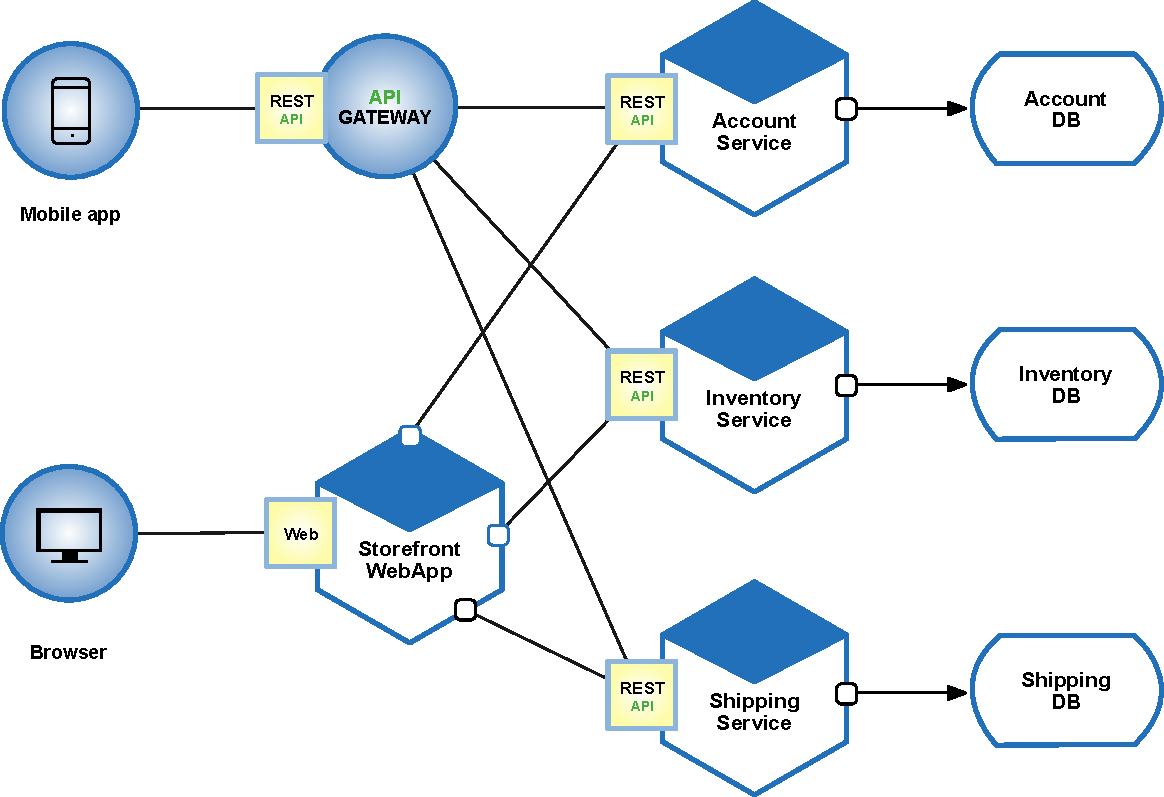
\includegraphics[width=.95\textwidth]{res/img/MS_architecture.pdf}
      \caption{Eine typische Microservice-Architektur eines fiktiven E-Commerce Systems \parencite{richardson2019msarchitecture}}
      \label{fig:microservice_architecture}
    \end{figure}

    %Vor- und Nachteile von Microservices
    Wie vorhin beschrieben, bieten Microservices auch eine Vielzahl an Vor- und Nachteilen, welche für eine Softwarearchitektur vor der Implementierung abgewägt werden müssen. Folgende Punkte definieren die Vorteile von Microservices:
    \begin{itemize}
      \item \textbf{Technische Heterogenität:} Bei einer Microservice-Architektur ist man nicht auf eine einzige Programmiersprache angewiesen. Da jeder Service seine eigene Laufzeitumgebung besitzt, kann pro Service eine andere Programmiersprache genutzt werden, solange diese über eine Kommunikationsschnittstelle wie beispielsweise \gls{ac-rest} einen Servicevertrag bereitstellen kann. Diesen Stil zum Schreiben von Software nennt man auch \emph{Polyglot Programming}, also mehrsprachiges Programmieren. Der Grundgedanke ist hierbei, dass man eine bestimmte Programmiersprache für einen bestimmten Anwendungsfall benutzt.
      
      Entwickelt man zum Beispiel eine Software auf Basis der Microservice-Architektur, die unter anderem ressourcenintensive Bildverarbeitungsalgorithmen nutzt, so könnte man einen Service definieren, der über Webtechnologien wie \emph{JavaScript} ankommende Bilddaten annimmt und an einen \emph{Bildverarbeitungs-Service} weitergibt, indem diese dann mithilfe von \emph{C++} oder \emph{Rust} performant verarbeitet werden. Die Sprachen C++ und Rust eignen sich hierbei zum Verarbeiten von Bilddaten, da diese hardwarenah ausgeführt werden, während sich JavaScript in der Webentwicklung etabliert hat.
      
      Dieser Vorteil bietet also eine Flexibilität beim Entwickeln von Services, da man je nach Anwendungsbereich der entwickelten Software verschiedene Services mit verschiedenen Programmiersprachen und deren jeweiligen Vorteilen nutzen kann.

      \item \textbf{Zuverlässigkeit:} In einer monolithischen Software beeinflusst jeder Teilbereich des Monolithen jeden anderen. Aus diesem Grund kann auch die gesamte Software fehlschlagen, sobald ein Teilbereich fehlschlägt. Bei einer Microservice-Architektur sind allerdings alle Teilbereiche voneinander abisoliert. Wenn in dem genannten Beispiel der Bildverarbeitungs-Service abstürzt, kann der \emph{Annahme-Service} noch auf \gls{ac-http}-Anfragen antworten und den Nutzer mit nötigen Informationen über das System versorgen. In der Zwischenzeit könnte dann eine neue Instanz des Bildverarbeitungs-Service gestartet werden. Dadurch wird ein System widerstandsfähig und zuverlässig.
      
      Um allerdings in den Genuss des Vorteils der Zuverlässigkeit von Microservices zu kommen, müssen neue Hürden überwunden werden. Diese äußern sich unter anderem in Form von Netzwerkkomplikationen bei der \emph{Inter-Service-Kommunikation}.

      \item \textbf{Skalierbarkeit:} Wie schon in \autoref{fig:monservscaling} dargestellt, muss bei einer hohen Auslastung einer monolithischen Webapplikation die komplette Applikation skaliert werden. Dies sorgt dafür, dass auch Module skaliert werden, die keine hohe Auslastung haben, aber ressourcenintensiv sind.
      
      Microservices hingegen können pro Service skaliert werden. Wenn also in dem Beispiel der Bildverarbeitung der C++- oder Rust-Service derzeit mit einer Prozessierung von Bilddaten ausgelastet ist, kann eine weitere Instanz dieses Service gestartet werden, der weitere Bilddaten entgegennehmen kann. Solange der JavaScript-Service nicht mit \gls{ac-http}-Anfragen ausgelastet ist, braucht dieser nicht zu skalieren. Dies erhöht die Ressourceneffizienz und auch die Kostenoptimierung eines Systems.

      \item \textbf{Leichte Installationen:} Mit einem wachsenden Monolithen wird es zunehmend schwerer einen solchen auf einer Maschine ohne Probleme zu installieren. Selbst eine einzige veränderte Zeile Code führt dazu, dass die komplette Applikation wieder kompiliert und installiert werden muss.
      \clearpage

      Bei Microservices stellt sich dieses Problem nicht, da diese als eigenständige Systeme zu betrachten sind. Wenn in dem obigen Beispiel der Bildverarbeitungs-Service ein Update benötigt, kann dieser unabhängig von dem JavaScript-Service aktualisiert werden.

      \item \textbf{Innovation:} Eine Microservice-Architektur vereinfacht das Einführen von neuen Technologie-Stacks und Frameworks, da jeder Service für sich steht. Gleichzeitig kann so ein vielversprechend aussehendes, aber möglicherweise riskantes Framework in einem Service zur Probe eingesetzt werden. Für den Fall, dass das Framework nicht die Anforderungen erfüllt, kann ein anderer Service mit einem anderen Framework eingesetzt werden.
      
      \item \textbf{Gesetz von Conway:} Wenn ein System in Microservices unterteilt ist, kann ein Entwicklerteam mit wenig Personal für jenes System einfacher eingeteilt werden. Dies führt zu effizienteren Kommunikationswegen und mehr Flexibilität im Unternehmen und der entwickelten Software.
      
      \item \textbf{Einfache Benutzbarkeit:} Ein Microservice legt eine primitive API offen, die durch festgelegte Operationen einfach zu benutzen ist. Diese Simplizität lädt andere Entwickler dazu ein, die API zu nutzen statt eine ähnliche Funktionalität zu entwickeln.
      
      \item \textbf{Effiziente Entwicklung:} Ein Service kann effizienter entwickelt werden, da dieser nur einen Bruchteil der Geschäftslogik widerspiegeln muss. Dadurch können Services mit relativ wenig Entwicklungszeit relativ viel Umsatz hervorrufen.
      
      \item \textbf{Automatisches Testen:} Ein Microservice kann durch seinen Minimalismus einfach getestet werden. Tests lassen sich in den jeweiligen Teilbereichen des entwickelten Systems detaillierter definieren, was eine erhöhte Qualität der Services hervorruft.
      
      \item \textbf{Effiziente Betreibbarkeit:} Ein Service kann durch seine geringe Komplexität einfach betrieben werden. Mittels einer funktionalen Virtualisierung oder Containerisierung, wie sie in \autoref{sec:container_vs_virtual_machines} behandelt wird, fügt dem Ganzen eine effizientere Installationsmöglichkeit hinzu.
    \end{itemize}
    \parencites[S. 21--22]{takai2017architektur}{newman2015buildingmicroservices}{allspaw2010web}[S. 23--25]{gallipeau2018microservices}
    \clearpage

    Microservices sind zwar ein neuer Ansatz, jedoch keine globale Lösung zum Entwickeln von Software. Diese bieten zwar viele Vorteile, enthalten allerdings auch einige Nachteile, welche im Folgenden aufgelistet sind:
    \begin{itemize}
      \item \textbf{Latenz:} Da Services in eigenen Laufzeitumgebungen im Netzwerk verteilt sind, entsteht in der Interkommunikation dieser eine erhöhte Latenz. Dadurch kann das System langsamer erscheinen. Bei Software mit regelmäßigen und vielen \gls{ac-http}-Anfragen kann das Nutzererlebnis gestört werden.
      
      \item \textbf{Netzwerkkomplikationen:} Ein verteiltes System ist niemals fehlerlos. Microservices sollten immer mit dem Gedanken entwickelt werden, dass deren Operationen fehlschlagen und dementsprechend gehandelt werden muss. Durch das Hinzukommen der \emph{Inter-Service-Netzwerkkomponente} können in einem verteilten System mehr Fehlersituationen entstehen als bei einem Monolithen.
      
      \item \textbf{Referenzielle Integrität:} Durch die Trennung der Datenbanken unter den Microservices kann die \emph{referenzielle Integrität} nicht gewahrt werden. Diese besagt, dass nur Entitäten mit einer Referenz auf einer weiteren Entität in einer Datenbank abgespeichert werden können, wenn dieser Eintrag auch in dieser Datenbank einmalig existiert. Auf die referenzielle Integrität muss also manuell geachtet werden.
      
      \item \textbf{Neues Paradigma:} Aufgrund dessen, dass die Microservice-Architektur ein relativ neues Thema in der Softwareentwicklung ist, müssen Entwicklerteams sich neue Kompetenzen aneignen. Zwar verringern Microservices durch das Abkapseln ihrer Geschäftslogik in kleine Teil-Services deren Komplexität, jedoch entsteht dadurch eine höhere Komplexität im Komponieren dieser Services. Die Komplexität des \gls{gl-devops}-Bereichs wird erhöht und muss von Entwicklerteams beachtet werden.
    \end{itemize}
    \parencite[S. 22]{takai2017architektur}

    %% Schluss
    % Erklärung, dass Microservices genutzt werden -> Argumente anhand von Vorteile Microservices
    Zum Öffnen der \gls{gl-onpremise} Software namens Royal Render, sodass diese remote-basiert benutzt werden kann, wird in dieser Arbeit eine Microservice-Architektur angestrebt. Für den zu entiwckelnden Remote-Controller wäre eine monolithische Architektur bei einer relativ kleinen Codebasis vollkommen legitim. Allerdings können die oben genannten Vorteile schon im Vorfeld auf das zu entwickelnde System abgebildet werden. Beispielsweise ist es nötig einen \emph{File-Service} zu entwickeln, der gewisse Datenmengen in einem Dateisystem hinterlegen kann. Durch lang andauernde Datenübertragungen muss der Service länger einen Zustand bewahren, was darauf schließen lässt, dass es wichtig ist, dass dieser Service unabhängig von dem Rest der Software skaliert werden kann, damit die Software reaktiv bleibt. Royal Render bietet deutlich mehr Features, die durch Royal Render-Anbindungen genutzt werden können. Es ist somit zu erwarten, dass die Software später mit mehr Services erweitert werden soll. Somit könnten die Features von Royal Render möglichst weitläufig und genau zur remote-basierten Nutzung abgedeckt und bereitgestellt werden.